\setlength{\columnsep}{3pt}
\begin{flushleft}
	Commands to kill a process:
	\begin{itemize}
		\item \textbf{kill}: Kills a specific process by sending some signal to it.
		\begin{tcolorbox}[breakable,notitle,boxrule=-0pt,colback=pink,colframe=pink]
			\color{black}
			\fontdimen2\font=9pt
			Syntax: kill [options] [process\_id]
			\fontdimen2\font=4pt
		\end{tcolorbox}
		Eg: Start a process and kill it with it's PID.
			\begin{figure}[h!]
				\centering
				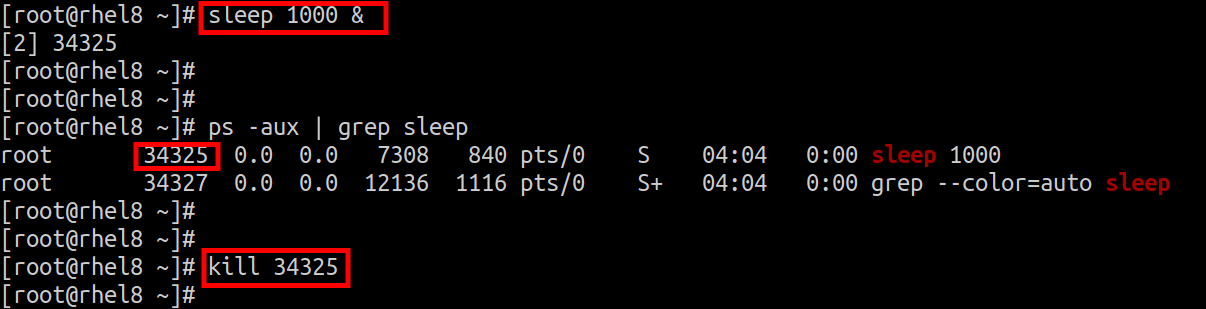
\includegraphics[scale=.3]{content/chapter12/images/kill1.png}
				\caption{Sample output}
				\label{fig:process23482}
			\end{figure}

		
		Options with \textbf{kill} command:	
		\begin{itemize}
			
			\item \textbf{-l}: List all signal associated with kill command.			
			\begin{tcolorbox}[breakable,notitle,boxrule=-0pt,colback=pink,colframe=pink]
				\color{black}
				\fontdimen2\font=9pt
				Syntax: kill -l
				\fontdimen2\font=4pt
			\end{tcolorbox}
			Eg: 
			\begin{figure}[h!]
				\centering
				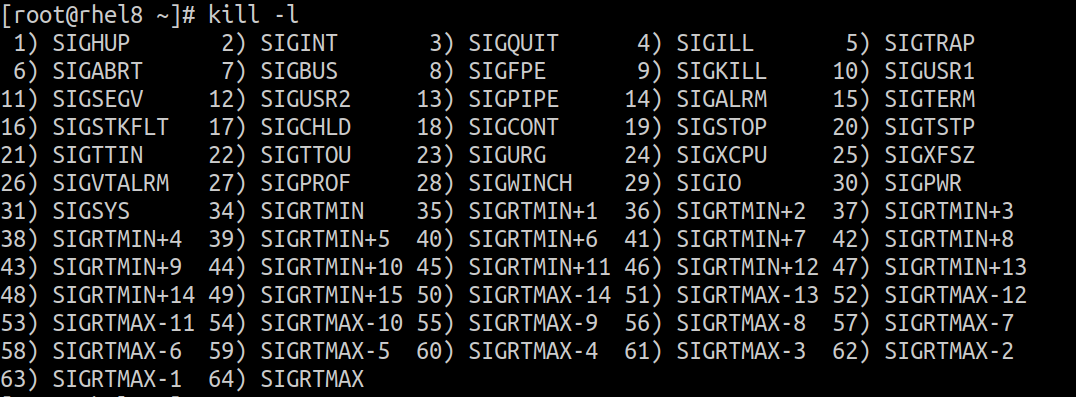
\includegraphics[scale=.3]{content/chapter12/images/kill2.png}
				\caption{Sample output}
				\label{fig:process2347}
			\end{figure}
			\newpage

			\item \textbf{-signal\_number}: Supply signal while killing a process.
			\begin{tcolorbox}[breakable,notitle,boxrule=-0pt,colback=pink,colframe=pink]
				\color{black}
				\fontdimen2\font=9pt
				Syntax: kill -signal\_number process\_id
				\fontdimen2\font=4pt
			\end{tcolorbox}		
			Eg:
			\begin{figure}[h!]
				\centering
				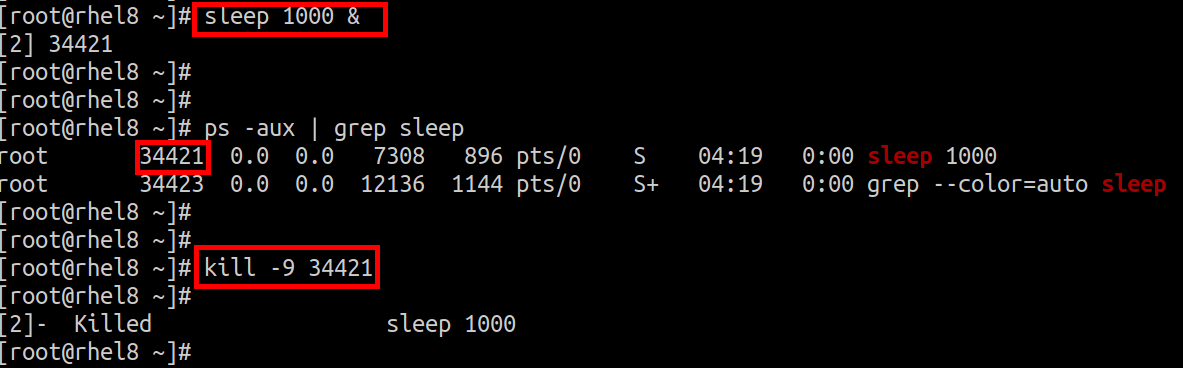
\includegraphics[scale=.25]{content/chapter12/images/kill3.png}
				\caption{Sample output}
				\label{fig:process23456}
			\end{figure}
		
			Meaning of some important signals:
			\begin{itemize}
				\item \textbf{SIGHUP (1)}: 
				\begin{itemize}
					\item Process hang due to death of controlling process.
					\item Eg:
					\begin{tcolorbox}[breakable,notitle,boxrule=-0pt,colback=black,colframe=black]
						\color{green}
						\fontdimen2\font=9pt
						\# sleep 6000 \&
						\newline
						\color{white}
						[1] 421019
						\newline
						\newline
						\color{green}						
						\# kill -1 421019
						\fontdimen2\font=4pt
					\end{tcolorbox}
				\end{itemize}
				\item \textbf{SIGINT (2)}: 
				\begin{itemize}
					\item Issued if the user sends an interrupt signal (Ctrl + C).
					\item Eg:
					\begin{tcolorbox}[breakable,notitle,boxrule=-0pt,colback=black,colframe=black]
						\color{green}
						\fontdimen2\font=9pt
						\# sleep 6000 \&
						\newline
						\color{white}
						[1] 421019
						\newline
						\newline
						\color{green}						
						\# kill -2 421019
						\newline
						\color{white}
						[1]+  Interrupt               sleep 6000
						\fontdimen2\font=4pt
					\end{tcolorbox}
				\end{itemize}
				\newpage
				\item \textbf{SIGQUIT (3)}: 
				\begin{itemize}
					\item Issued if the user sends a quit signal (Ctrl + D).
					\item Eg:
					\begin{tcolorbox}[breakable,notitle,boxrule=-0pt,colback=black,colframe=black]
						\color{green}
						\fontdimen2\font=9pt
						\# sleep 6000 \&
						\newline
						\color{white}
						[1] 421019
						\newline
						\newline
						\color{green}						
						\# kill -3 421019
						\newline
						\color{white}
						[1]+  Quit              (core dumped) sleep 6000
						\fontdimen2\font=4pt
					\end{tcolorbox}
				\end{itemize}
			\item \textbf{SIGKILL (9)}: 
			\begin{itemize}
				\item If a process gets this signal it must quit immediately and will not perform any clean-up operations.
				\item Eg:
				\begin{tcolorbox}[breakable,notitle,boxrule=-0pt,colback=black,colframe=black]
					\color{green}
					\fontdimen2\font=9pt
					\# sleep 6000 \&
					\newline
					\color{white}
					[1] 421019
					\newline
					\newline
					\color{green}						
					\# kill -9 421019
					\newline
					\color{white}
					[1]+  Killed                  sleep 6000
					\fontdimen2\font=4pt
				\end{tcolorbox}
			\end{itemize}
		
			\item \textbf{SIGTERM (15)}: 
			\begin{itemize}
				\item Software termination signal (sent by kill by default).
				\item Eg:
				\begin{tcolorbox}[breakable,notitle,boxrule=-0pt,colback=black,colframe=black]
					\color{green}
					\fontdimen2\font=9pt
					\# sleep 6000 \&
					\newline
					\color{white}
					[1] 421019
					\newline
					\newline
					\color{green}						
					\# kill -15 421019
					\newline
					\color{white}
					[1]+  Killed                  sleep 6000
					\fontdimen2\font=4pt
				\end{tcolorbox}
			\end{itemize}
			\newpage
			\item \textbf{SIGSTOP (19)}: 
			\begin{itemize}
				\item Issued if the user sends a stop signal (Ctrl + Z).
				\item Eg:
				\begin{tcolorbox}[breakable,notitle,boxrule=-0pt,colback=black,colframe=black]
					\color{green}
					\fontdimen2\font=9pt
					\# sleep 6000 \&
					\newline
					\color{white}
					[1] 421019
					\newline
					\newline
					\color{green}						
					\# kill -19 421019
					\newline
					\color{white}
					[1]+  Stopped                 sleep 6000
					\fontdimen2\font=4pt
				\end{tcolorbox}
			\end{itemize}

			\item \textbf{SIGCONT (18)}: 
			\begin{itemize}
				\item Issued if the user sends a resume signal.
				\item Eg:
				\begin{tcolorbox}[breakable,notitle,boxrule=-0pt,colback=black,colframe=black]
					\color{green}
					\fontdimen2\font=9pt
					\# sleep 6000 \&
					\newline
					\color{white}
					[1] 421019
					\newline
					\newline
					\color{green}						
					\# kill -18 421019
					\newline
					\# jobs
					\newline
					\color{white}
					[1]+  Running                 sleep 6000 \&
					\fontdimen2\font=4pt
				\end{tcolorbox}
			\end{itemize}

		
			\end{itemize}
		

					
		\end{itemize}
	
	\newpage
	\item \textbf{killall}: Kill multiple running process by process name instead of it's process ID. Zombie process needs to be killed using process name as they won't have process ID.
	\bigskip
	\begin{tcolorbox}[breakable,notitle,boxrule=-0pt,colback=pink,colframe=pink]
		\color{black}
		\fontdimen2\font=9pt
		Syntax: killall [options] process\_name
		\fontdimen2\font=4pt
	\end{tcolorbox}
	Eg:
	\begin{figure}[h!]
		\centering
		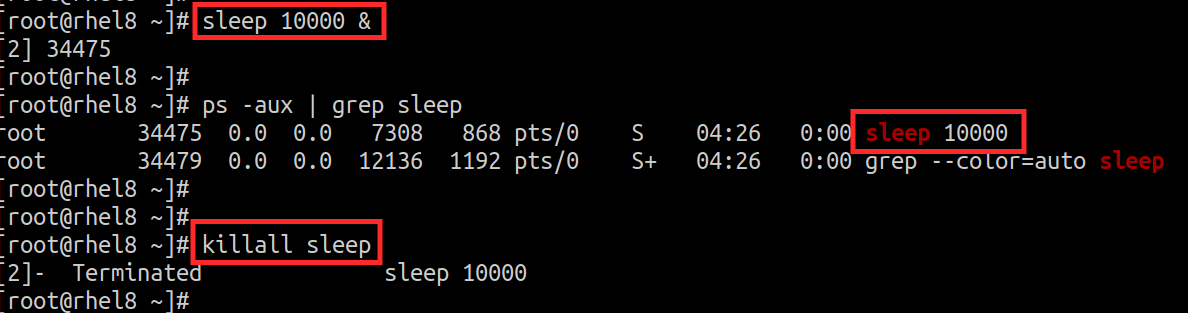
\includegraphics[scale=0.25]{content/chapter12/images/kill4.png}
		\caption{Sample output}
		\label{fig:top_command_output5}
	\end{figure}

	\item \textbf{pkill}: The pkill command, like killall, can signal multiple processes.
	\bigskip
	\begin{tcolorbox}[breakable,notitle,boxrule=-0pt,colback=pink,colframe=pink]
		\color{black}
		\fontdimen2\font=9pt
		Syntax: pkill process\_name
		\fontdimen2\font=4pt
	\end{tcolorbox}
	Eg:
	\begin{tcolorbox}[breakable,notitle,boxrule=-0pt,colback=black,colframe=black]
		\color{green}
		\fontdimen2\font=9pt
		\# pkill sleep
		\fontdimen2\font=4pt
	\end{tcolorbox}

		
	\end{itemize}

\end{flushleft}

\newpage


